\section{Inleiding}

In dit document wordt behandeld hoe de testkast werkt en hoe deze te bedienen is. Daarnaast zijn er een aantal dingen die er fout kunnen gaan. Dit document gaat hier verder op in en wat er gedaan kan worden in deze gevallen. De software op de testkast is in tegenstelling tot de vorige software niet alleen maar in \gls{TwinCAT} geschreven. De frontend \gls{gui} (wat je ziet) is net als in VACAM een apart programma en communiceert via \gls{ADS} met de backend \gls{PLC} (TwinCAT dus). Het voordeel hiervan is dat \gls{TwinCAT} gemanipuleerd kan worden vanaf de frontend en dat de \gls{gui} niet hoeft te sluiten bij het herstarten van \gls{TwinCAT}. De structuur van zowel de frontend als de backend zijn vergelijkbaar met hoe VACAM is geschreven om onderhoud gebruiksvriendelijk te houden.

\begin{figure}[H]
	\centering
	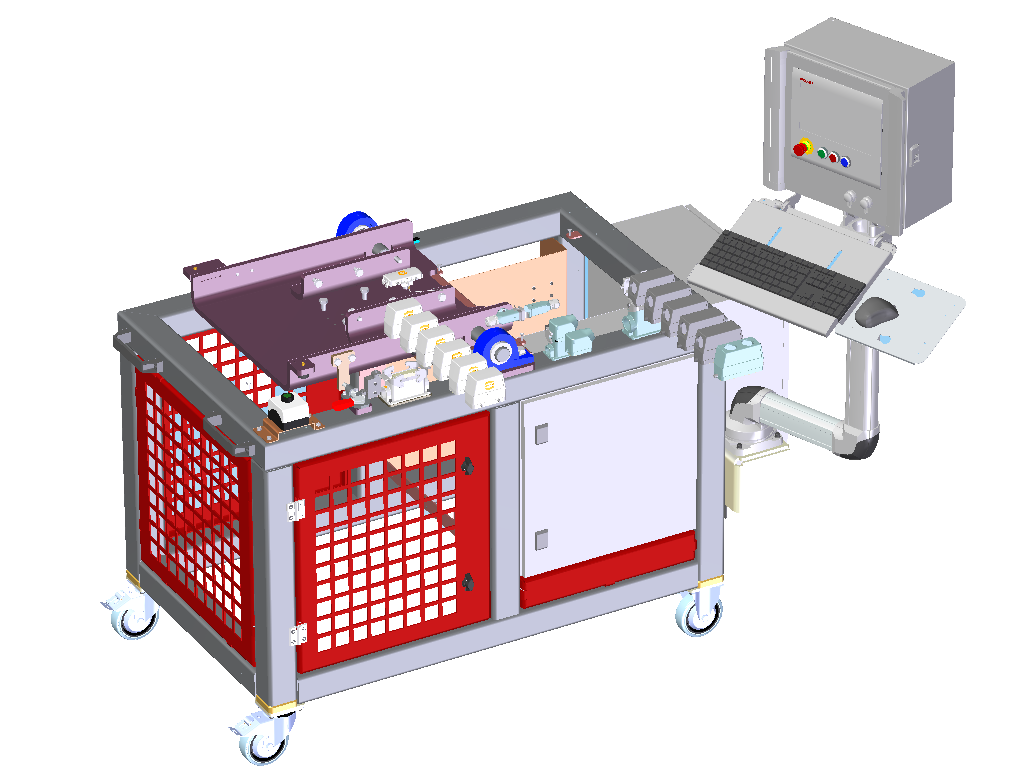
\includegraphics[width=\linewidth]{TestkastDrawing}
	\label{fig:TestkastDrawing}
	\caption{3D model van de testkast}
\end{figure}